\documentclass{emulateapj}
%\documentclass[12pt,preprint]{aastex}

\usepackage{graphicx}
\usepackage{float}
\usepackage{amsmath}
\usepackage{epsfig,floatflt}
\usepackage{url}
\usepackage[caption=false]{subfig}
\usepackage{url}
\setcitestyle{square}




\begin{document}

\title{Project 4}

\author{Christer Dreierstad}

\email{chrisdre@student.matnat.uio.no}

\altaffiltext{1}{Institute of Physics, University of
  Oslo, P.O.\ Box 1029 Blindern, N-0315 Oslo, Norway}


%\date{Received - / Accepted -}

\begin{abstract}
In this study of phase transformations of a magnetic system we will estimate the critical temperature using the Ising model. To study the system of time we will use the Metropolis algorithm, which is a Markov chain-Monte Carlo method. Since we do not know all the possible states of the system beforehand, the Metropolis algorithm is beneficial to use, since it eliminates the partition function. The study will show that for a cold system of temperature 1 kT/J the system rarely has states of higher energies, when increasing the temperature to 2.4 kT/J the total energy of the system is increased, and we see that the probability for the system to be in a higher energy state is increased. When we look at how the system evolve as a function of temperature we clearly see that there is a phase transformation at a temperature close to the critical temperature. When estimating the critical temperature we find this to be $T_C = 2.256$ kT/J, which is fairly close to the analytical value found by Lars Onsager \cite{bib:onsager}.

\end{abstract}
\keywords{computational science: Ising model  --- methods: Metropolis algorithm, Markov chain-Monte Carlo}

\section{Introduction}
\label{sec:introduction}
To study the phase transitions of a magnetic system we consider the Ising model for a two-dimensional system with a finite lattice size. The particles (spins) that make up the crystal (lattice) can take two values representing spin up or down. The energy of the lattice can then, by the Ising model, be found by
%
\begin{gather}\label{eq:energyIsing}
    E = -J\sum_{< kl >}^N s_k s_l,
\end{gather}
%
when there is no external magnetic field applied to the system.  The coupling constant J will be set to 1, which means we are studying a ferromagnetic interaction between the spins that make up the lattice. Since the coupling constant is dependent upon the material we study, setting this to 1 allows for a general model. For studying the phase transition we use a Markov chain Monte Carlo method (MCMC), and the probability of finding the system in a given state $i$ is
%
\begin{align}\label{eq:P_i}
    P_i = P(E_i) = \frac{e^{-\beta E_i}}{Z},
\end{align}
%
where Z is the partition function $Z = \sum_i e^{-\beta E_i}$, which is impossible to calculate unless we know all the states. To eliminate the partition function we will use the Metropolis algorithm, which eliminates the partition function. When applying the algorithm we will consider periodic boundary conditions of the lattice, which will allow us to simulate an infinitely large lattice, and we do not have to consider what happens on the boundary the lattice (the ends of the material). Increasing the size of the lattice will further improve the approximation of a large scale lattice. The goal of the MCMC simulation is to observe the energy and the magnetic moment as time (MC cycles) increase, we expect the system to stabilize in the most probable state.


\section{Method}
\subsection{Analytical expressions}
\label{sec:method}
\begin{deluxetable}{cccc}
\tablewidth{0pt}
\tablecaption{\label{tab:energies}}
\tablecomments{States of the 2x2 lattice and corresponding values for energy and magnetic moment. Notice that the ground state (the lowest energy) has either all spins pointing up or down.}
\tablecolumns{4}
\tablehead{Spins up  & Degeneracy & Energy & Magnetic moment}
\startdata
4 & 1 & -8J & 4 \\
3 & 4 & 0 & 2 \\
2 & 4 & 0 & 0 \\
2 & 2 & 8J & 0 \\
1 & 4 & 0 & -2 \\
0 & 1 & -8J & -4
\enddata
\end{deluxetable}

The two-dimensional binary Ising model has analytical expectation values. The partition function
%
\begin{equation*}
    z = \sum_i \Omega(E_i) e^{\beta E_i},
\end{equation*}
%
where $\Omega(E_i)$ is the degeneracy of energy $E_i$ and $\beta = 1/k_BT$. From Table \ref{tab:energies} we can see that there are 2 energies that are non-zero: $\pm 8J$, which both has a degeneracy of 2. The energy equal to zero has a degeneracy of 12. Expanding the sum of the partition function we get 
%
\begin{align*}
    z &= 2e^{8J\beta} + 12 + 2e^{-8J\beta} \\
    &= 12 + 2\left(e^{8J\beta} + e^{-8J\beta}\right),
\end{align*}
%
where we have inserted $e^0 = 1$. We know that $\cosh(x) = \frac{1}{2}\left( e^{-x} + e^x\right)$, inserting this gives
%
\begin{gather}\label{eq:z}
    Z = 12 + 4\cosh(8J\beta).
\end{gather}
%
The mean value of the energy is given by
%
\begin{align*}
    \langle E \rangle = -\frac{\partial }{\partial \beta} \ln Z = -\frac{1}{Z}\frac{\partial Z}{\partial \beta},
\end{align*}
%
which is found by inserting the partition function.
%
\begin{align*}
    \langle E \rangle &= -\frac{1}{Z}\frac{\partial}{\partial \beta} \left(12 + 4 \cosh\left(8J\beta\right)\right)\\
    &= -\frac{4}{Z}\left(8J\sinh\left(8J\beta\right)\right),
\end{align*}
pulling a factor 4 from the partition function and inserting we are left with a analytical solution to the mean energy of the lattice
%
\begin{gather*}
    \langle E \rangle = -\frac{8J\sinh\left(8J\beta\right)}{3 + \cosh(8J\beta}.
\end{gather*}
%
The heat capacity can be found by
%
\begin{align*}
    C_V &= \frac{1}{kT^2}\frac{\partial^2}{\partial \beta^2} \ln Z = \frac{1}{kT^2}\frac{\partial}{\partial \beta}\left(\frac{\partial}{\partial \beta} \ln Z\right),
\end{align*}
%
where we recognize the partial derivative in the parenthesis as the negative mean energy. 
%
\begin{align*}
    C_V = \frac{1}{kT^2}\bigg(&\frac{64J^2\cosh\left(8J\beta\right)\left(3 + \cosh\left(8J\beta\right)\right)}{\left(3 + \cosh\left(8J\beta\right)\right)^2} \\ &-\frac{64J^2\sinh^2\left(8J\beta\right)}{\left(3 + \cosh\left(8J\beta\right)\right)^2}\bigg),
\end{align*}
%
by inserting for the mean energy and using the product rule. Further simplifications gives the mean heat capacity
%
\begin{gather*}
    C_V = \frac{64J^2}{k_B T^2} \left(\frac{\cosh(8\beta J)(3+\cosh(8 \beta J)) - \sinh^2(8\beta J)}{\left(3 + \cosh(8\beta J)\right)^2}\right)
\end{gather*}
The susceptibility is given as
%
\begin{equation*}
    \chi = \frac{1}{kT}\left(\langle M^2 \rangle - \langle M \rangle^2\right).
\end{equation*}
%
To find the susceptibility of the system we consider the mean magnetic moment
%
\begin{equation*}
    \langle M \rangle = \frac{1}{Z} \sum_i |M_i| e^{-\beta E_i},
\end{equation*}
where we find the magnetic moment for a given energy in Table \ref{tab:energies}. So the mean magnetic moment is
%
\begin{equation*}
    \langle M \rangle = \frac{1}{Z}\left(4e^{8J\beta} + 4\left(2e^{0}\right) + 4\left(-2e^0\right) + -4e^{8J\beta} \right) = 0.
\end{equation*}
%
Further we calculate the mean of the  magnetic moment squared
%
\begin{equation*}
    \langle M^2 \rangle = \frac{1}{Z}\sum_i M_i^2 e^{-\beta E_i},
\end{equation*}
and again referring to Table \ref{tab:energies} we get
%
\begin{align*}
    \langle M^2 \rangle &= \frac{1}{Z}\left(16\left(2e^{8J\beta}\right) + 16\left(2e^0\right) \right) \\
    &= \frac{8\left(e^{8J\beta} + 1\right)}{3 + \cosh\left(8J\beta\right)}.
\end{align*}
So the susceptibility of the system is given as
%
\begin{equation*}
    \chi = \frac{1}{kT^2}\langle M^2 \rangle = \frac{1}{kT^2}\frac{8\left(e^{8J\beta} + 1\right)}{3 + \cosh\left(8J\beta\right)}
\end{equation*}
%
Further we find the mean of the absolute value of the magnetic moment by

\begin{align*}
    \langle |M| \rangle &= \frac{1}{Z} \sum_i |M_i| e^{-\beta E_i} \\
     &= \frac{1}{Z}\left(4e^{8J\beta} + 4\left(2e^{0}\right) + 4\left(|-2|e^0\right) + |-4|e^{8J\beta} \right) \\
     &= \frac{2e^{8J\beta} + 4}{3 + \cosh\left(8J\beta\right)},
\end{align*}
%
after pulling out a factor 4 from the partition function. To summarize we have the following analytical expression for the system
%
\begin{align*}
    &\langle E \rangle = -\frac{4}{Z}\left(8J\sinh\left(8J\beta\right)\right), \\
    &\langle |M| \rangle = \frac{2e^{8J\beta} + 4}{3 + \cosh\left(8J\beta\right)}, \\
    &C_V = \frac{64J^2}{k T^2} \left(\frac{\cosh(8\beta J)(3+\cosh(8 \beta J)) - \sinh^2(8\beta J)}{\left(3 + \cosh(8\beta J)\right)^2}\right), \\
    &\chi = \frac{1}{kT^2}\frac{8\left(e^{8J\beta} + 1\right)}{3 + \cosh\left(8J\beta\right)}.
\end{align*}

\subsection{Ising model}
When the energy of the Ising model we consider the equation given in the introduction, Eq. \eqref{eq:energyIsing}, where the subscript of the sum means we are taking the sum over the neighbouring spins, N is the total amount of spins and $s_k$, $s_l = \pm 1$, represents the spin of the particles. Consider a random spin at the lattice, in the two-dimensional case it has a total of four neighbours that it interacts with.  An example for a spin surrounded by four spin up.
%
\begin{equation*}
    \begin{matrix}
    & \uparrow & \\
    \uparrow & \uparrow & \uparrow \\
    & \uparrow & \\
    \end{matrix},
   % \quad
    %\longrightarrow
    %\quad
    %\begin{matrix}
    %& \uparrow & \\
    %\uparrow & \uparrow & \uparrow \\
    %& \uparrow & \\
    %\end{matrix}
\end{equation*}
%
with energy $E = -4J$. Changing one of the spins in the example above results in a new configuration with a new energy and magnetic moment. Following are five examples that show the different energies $E = 0, \pm 2J, \pm 4J$, and the resulting energy when flipping the spin we are located at:

\begin{align*}
    E = -4J
    \quad
    \begin{matrix}
    & \uparrow & \\
    \uparrow & \uparrow & \uparrow \\
    & \uparrow & \\
    \end{matrix}
    \quad
    \Longrightarrow
    \quad
    E = 4J
    \quad
    \begin{matrix}
    & \uparrow & \\
    \uparrow & \downarrow & \uparrow \\
    & \uparrow & \\
    \end{matrix} \\
\end{align*}
where the change of energy $\Delta E = E_{after} - E_{before} = 8J$.
\begin{align*}
    E = -2J
    \quad
    \begin{matrix}
    & \uparrow & \\
    \downarrow & \uparrow & \uparrow \\
    & \uparrow & \\
    \end{matrix}
    \quad
    \Longrightarrow
    \quad
    E = 2J
    \quad
    \begin{matrix}
    & \uparrow & \\
    \downarrow & \downarrow & \uparrow \\
    & \uparrow & \\
    \end{matrix}
\end{align*}
with $\Delta E = 4J$.
\begin{align*}
    E = 0
    \quad
    \begin{matrix}
    & \uparrow & \\
    \downarrow & \uparrow & \uparrow \\
    & \downarrow & \\
    \end{matrix}
    \quad
    \Longrightarrow
    \quad
    E = 0
    \quad
    \begin{matrix}
    & \uparrow & \\
    \downarrow & \downarrow & \uparrow \\
    & \downarrow & \\
    \end{matrix}
\end{align*}
with $\Delta E = 0$.
\begin{align*}
    E = -2J
    \quad
    \begin{matrix}
    & \uparrow & \\
    \downarrow & \uparrow & \downarrow \\
    & \downarrow & \\
    \end{matrix}
    \quad
    \Longrightarrow
    \quad
    E = 2J
    \quad
    \begin{matrix}
    & \uparrow & \\
    \downarrow & \downarrow & \downarrow \\
    & \downarrow & \\
    \end{matrix}
\end{align*}
with $\Delta E = -4J$.
\begin{align*}
    E = 4J
    \quad
    \begin{matrix}
    & \downarrow & \\
    \downarrow & \uparrow & \downarrow \\
    & \downarrow & \\
    \end{matrix}
    \quad
    \Longrightarrow
    \quad
    E = -4J
    \quad
    \begin{matrix}
    & \downarrow & \\
    \downarrow & \downarrow & \downarrow \\
    & \downarrow & \\
    \end{matrix}
\end{align*}
with $\Delta E = -8J$. We now see that for a random spin of the lattice we have known values for the change of energy $\Delta E$. 

\subsection{Implementation}
For a MC cycle we initialize the lattice by setting all the spins in either a random or an ordered state, and then calculating the energy and the magnetic moment. We then iterate over the lattice at random positions (i.e. we check $L^2$ random spins), for each of these positions we calculate the change in energy $\Delta E$. Consider the ratio of the probability of the new energy $P\left(E_{new}\right)$ and the previous energy $P\left(E_{prev}\right)$:
%
\begin{align*}
    \frac{P\left(E_{new}\right)}{P\left(E_{prev}\right)} = \frac{e^{-\beta E_{new}}/Z}{e^{-\beta E_{prev}}/Z} = e^{-\beta\left(E_{new} - E_{prev}\right)} = e^{-\beta\Delta E},
\end{align*}
%
where Z is the the partition function. We now perform the Metropolis test for a given $\Delta E$;
%
\begin{equation*}
    r \leq e^{-\beta \Delta E}, \qquad r \in [0,1]
\end{equation*}
%
i.e. if the ratio is larger than or equal to a random number $r \in [0,1]$ we accept a new configuration, and flip the spin.  We are looking at the change in energy if we were to flip a random spin; if the change of energy is large, the likelihood of this spin being flipped is small, so we reject this solution, on the other hand, if the probability is large, we accept the configuration. Since we expect the system to move to more likely state, we are looking for states that does not increase the systems energy. A large change in energy means we are looking at a spin that has half or more of its surrounding spins in the same configuration, and the system seems to locally move towards a steady state, therefore the local system is not changed. For each such Metropolis test that succeeds we add the flip of spin as a contribution to the systems energy and magnetic moment. When the calculations over the lattice is complete we conclude a single MC cycle and store the final value for the energy and magnetic moment. When we are calculating the final mean values of the energy and magnetic moment, we ignore the first 5\% of the data, so we are not including the values before the system is in equilibrium.

\subsection{Critical temperature}
As the temperature of the system moves towards the critical temperature, the susceptibility $\chi$ and the heat capacity $C_V$ moves towards an infinite value. We can see this by
%
\begin{gather*}
    C_V \sim |T_C - T|^{-\alpha} \\
    \chi \sim |T_C - T|^{-\nu},
\end{gather*}
%
where $\alpha$ and $\nu$ are positive constants. For the results in this study we have clearer peaks for the susceptibility, so we will extract the critical temperature from these. We know that the critical tempeature scales as
%
\begin{gather*}
    T_C\left(L\right) - T_C\left(L=\infty\right) = aL^{-1/\nu},
\end{gather*}
where we set $\nu = 1$, and a is a positive constant. Solving the above equation for the critical temperature as the lattice size is infinite we get
%
\begin{gather*}
    T_C\left(L=\infty \right) \approx T_C\left(L\right) - \frac{1}{L}.
\end{gather*}




\section{Results}
\label{sec:results}
Following are the results produced in this study. The results are found in plots and tables, and the content is presented in the following subsections.

\subsection{Comparison of analytical and numerical values}
Table \ref{tab:numAnal} shows a comparison of analytical and numerical values for a 2x2 lattice. 

\begin{deluxetable}{lcccc}
\tablewidth{0pt}
\tablecaption{\label{tab:numAnal}}
\tablecomments{Comparison of analytical and numerical results for various MC cycles. Lattice size is 2x2, temperature 1 kT/J and initial spin randomly set.}
\tablecolumns{5}
\tablehead{MC cycles & $\langle E \rangle$ & $\langle |M| \rangle$ & $C_V$ & $\chi$}
\startdata
1e3 & -7.984 & 3.996 & 0.127 & 0.019 \\
5e3 & -7.985 & 3.994 & 0.114 & 15.916 \\
1e4 & -7.981 & 3.994 & 0.146 & 15.769 \\
1e5 & -7.984 & 3.994 & 0.129 & 15.847 \\
1e6 & -7.984 & 3.994 & 0.127 & 15.973 \\
Analytical & -7.983 & 3.994 & 0.128 & 15.973 
\enddata
\end{deluxetable}

\subsection{Mean energy and magnetisation 20x20 lattice}
Figures \ref{fig:L20-GS-E-T1} and \ref{fig:L20-GS-M-T1} shows the energy and magnetisation of the ground state for temperature 1 kT/J, while figures \ref{fig:L20-GS-E-T2.4} and \ref{fig:L20-GS-M-T2.4} shows the same for temperature 2.4 kT/J. We see that the system stabilizes quickly. For the non-ground state plots see figures \ref{fig:L20-E-T1} and \ref{fig:L20-M-T1} for temperature 1 kT/J and figures \ref{fig:L20-E-T2.4} and \ref{fig:L20-M-T2.4} for temperature 2.4 kT/J. For the system that starts in a random spin state we see by figure \ref{fig:EM-T1_zoom} that the system stabilizes at about 250 MC cycles.
%
\begin{figure}
\subfloat[Energy pr. spin.]{
  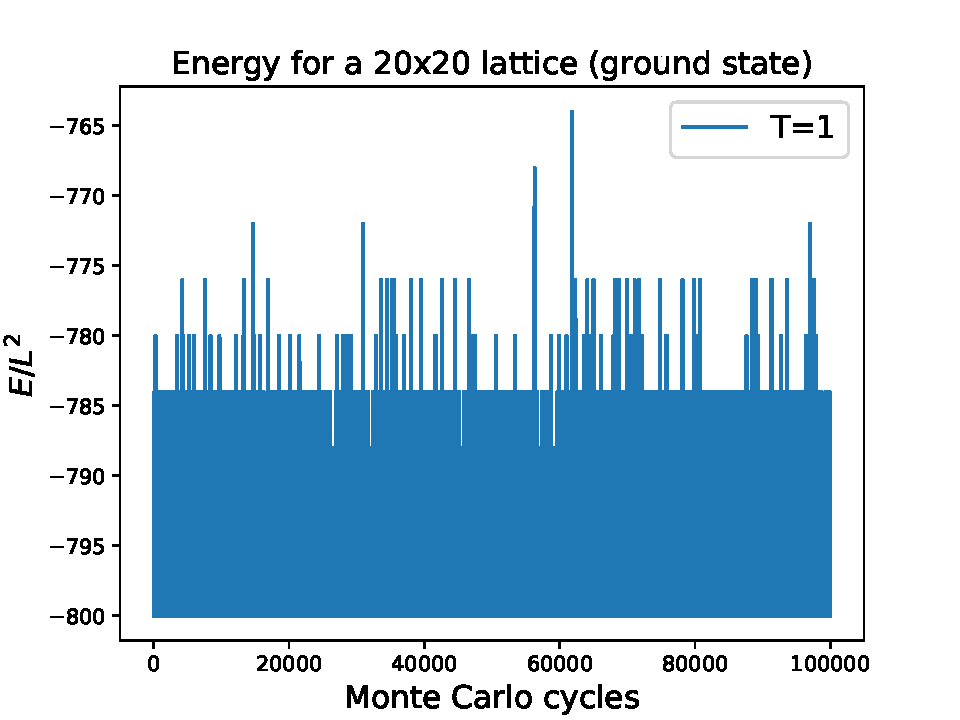
\includegraphics[width=8.65cm]{EofMCC-GS-T1-L20-1e5.pdf}
  \label{fig:L20-GS-E-T1}} \\
\subfloat[Absolute value of the magnetic moment pr. spin.]{
  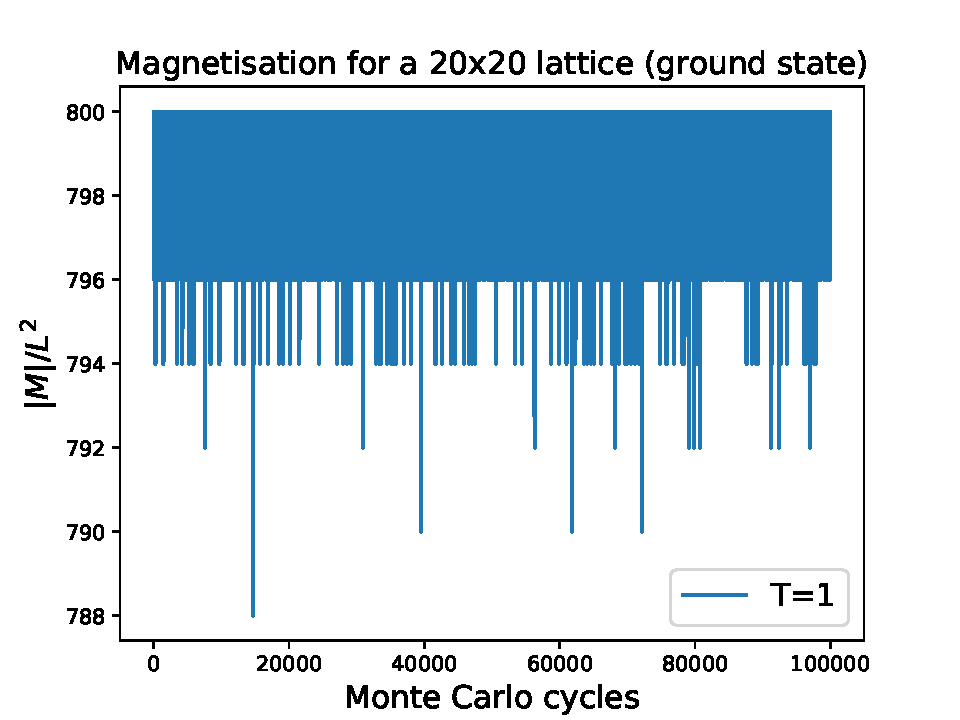
\includegraphics[width=8.65cm]{MofMCC-GS-T1-L20-1e5.pdf}
  \label{fig:L20-GS-M-T1}}
\caption{Time evolution (MC cycles) of energy and magnetic moment of an ordered initial state with temperature 1 kT/J. $10^5$ Monte Carlo cycles.}
\label{fig:EM-GS-T1}
\end{figure}
%
\begin{figure}
\subfloat[Energy pr. spin.]{%
  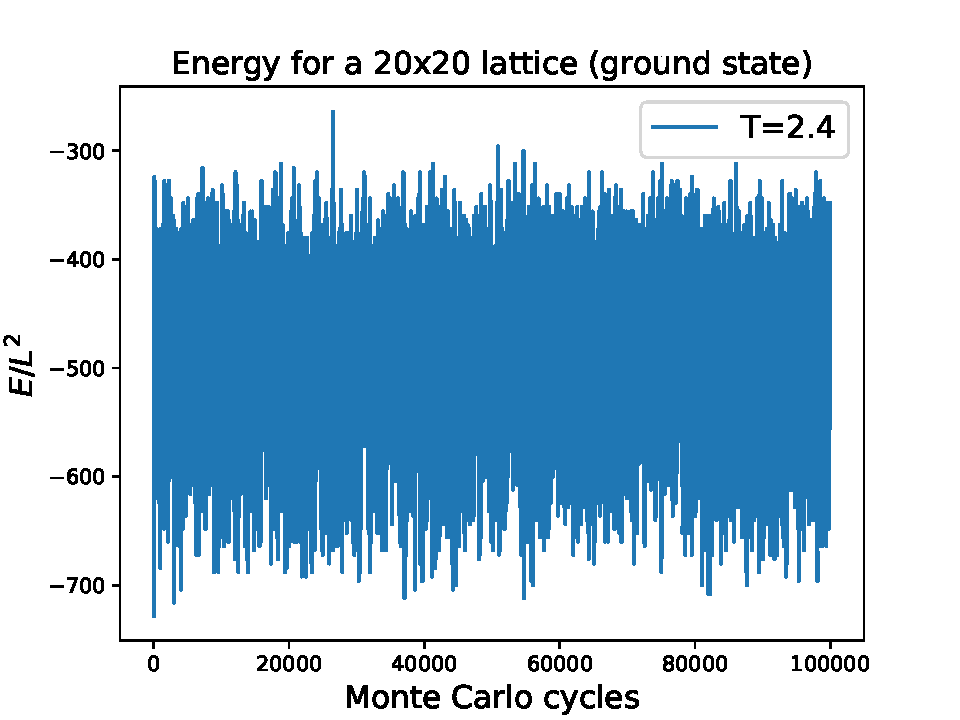
\includegraphics[width=8.65cm]{EofMCC-GS-T2_4-L20-1e5.pdf}
  \label{fig:L20-GS-E-T2.4}} \\
\subfloat[Absolute value of the magnetic moment pr. spin.]{
  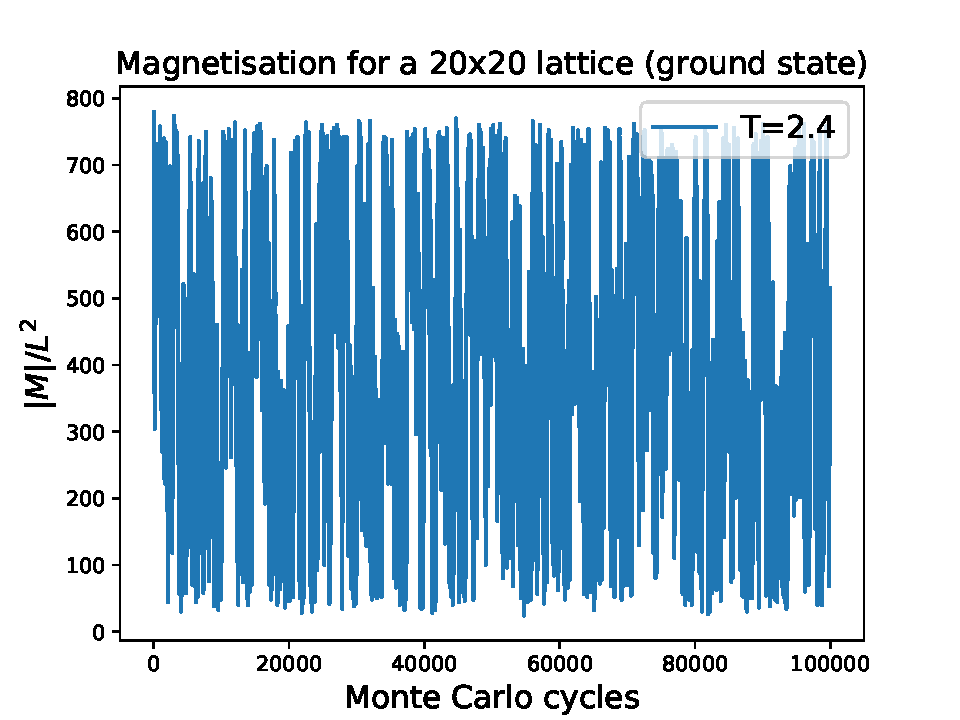
\includegraphics[width=8.65cm]{MofMCC-GS-T2_4-L20-1e5.pdf}
  \label{fig:L20-GS-M-T2.4}}
\caption{Time evolution of energy and magnetic moment of an ordered initial state with temperature 2.4 kT/J. $10^5$ Monte Carlo cycles.}
\label{fig:EM-GS-T2.4}
\end{figure}
%
\begin{figure}
\subfloat[Energy pr. spin.]{
  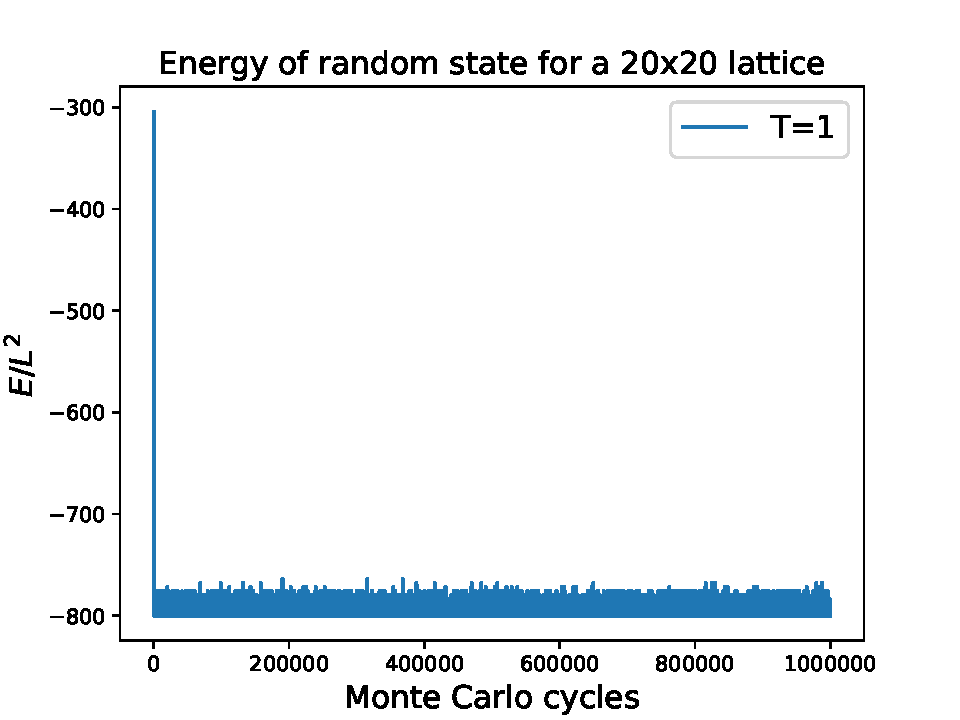
\includegraphics[width=8.65cm]{EofMCC-T1-L20-1e6.pdf}
  \label{fig:L20-E-T1}} \\
\subfloat[Absolute value of the magnetic moment pr. spin.]{%
  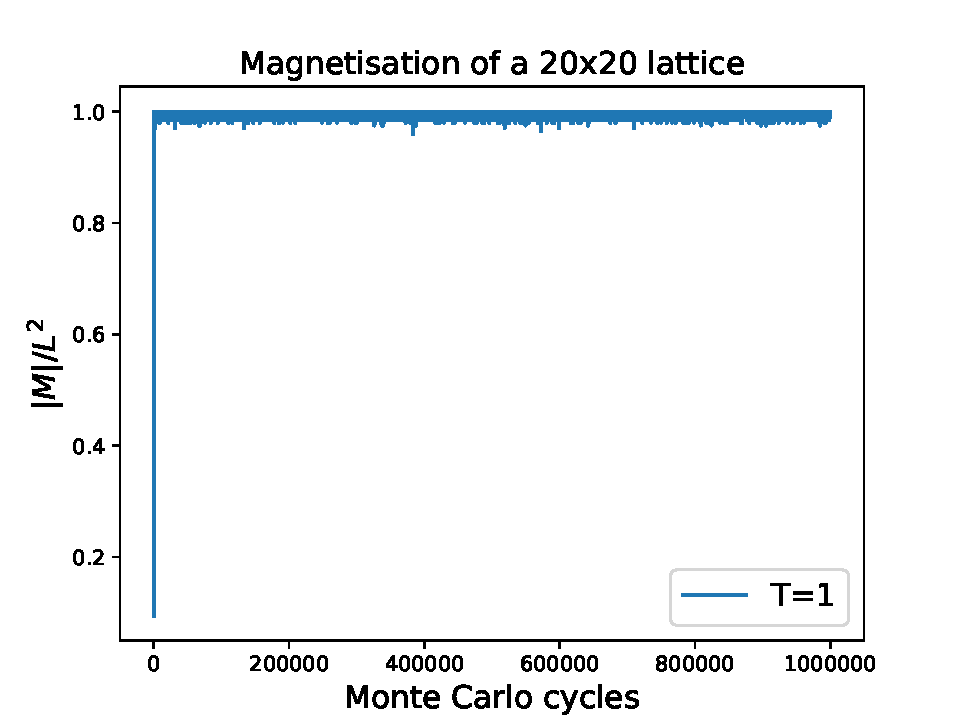
\includegraphics[width=8.65cm]{MofMCC-T1-L20-1e6.pdf}
  \label{fig:L20-M-T1}}
\caption{Time evolution of energy and magnetic moment of an random initial state with temperature 1 kT/J. $10^6$ Monte Carlo cycles.}
\label{fig:EM-T1}
\end{figure}
%
\begin{figure}
\subfloat[Zoom of figure \ref{fig:L20-E-T1}.]{
  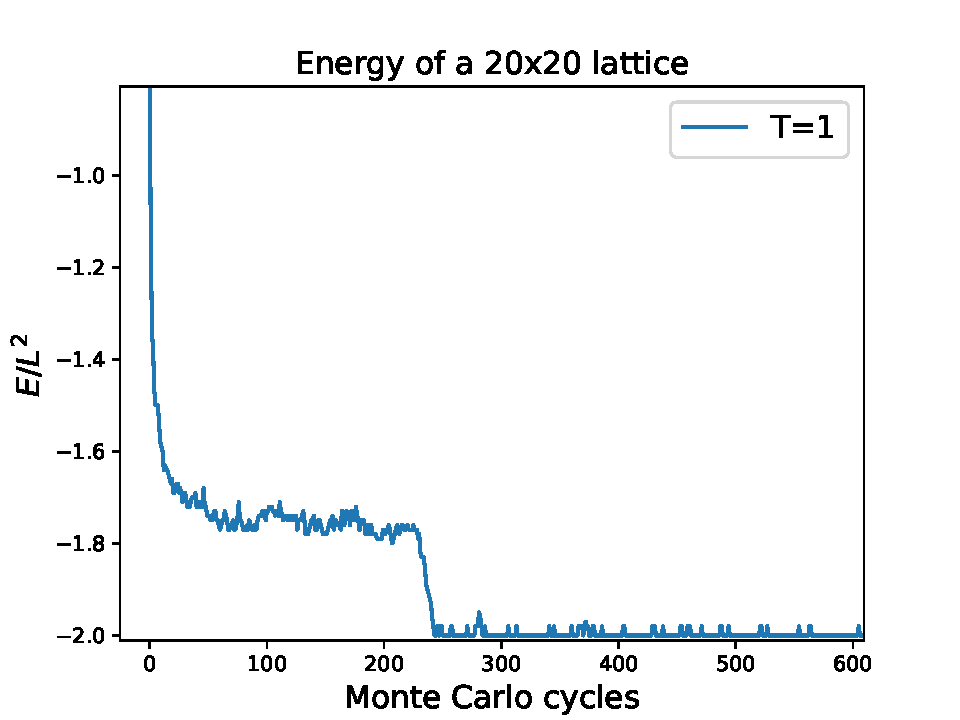
\includegraphics[width=8.65cm]{EofMCC-T1-L20-1e6_zoom.pdf}
  \label{fig:L20-E-T1_zoom}} \\
\subfloat[Zoom of figure \ref{fig:L20-M-T1}.]{%
  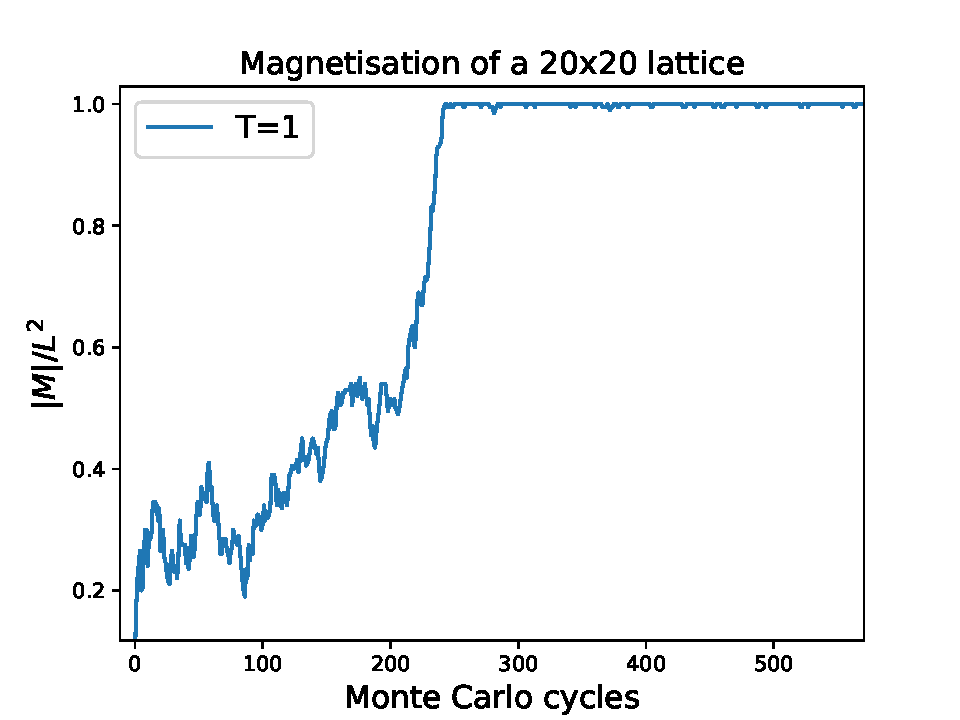
\includegraphics[width=8.65cm]{MofMCC-T1-L20-1e6_zoom.pdf}
  \label{fig:L20-M-T1_zoom}}
\caption{Zoom of previous plot to show where the energy and magnetisation stabilized.}
\label{fig:EM-T1_zoom}
\end{figure}
%
\begin{figure}
\subfloat[Energy pr. spin.]{
  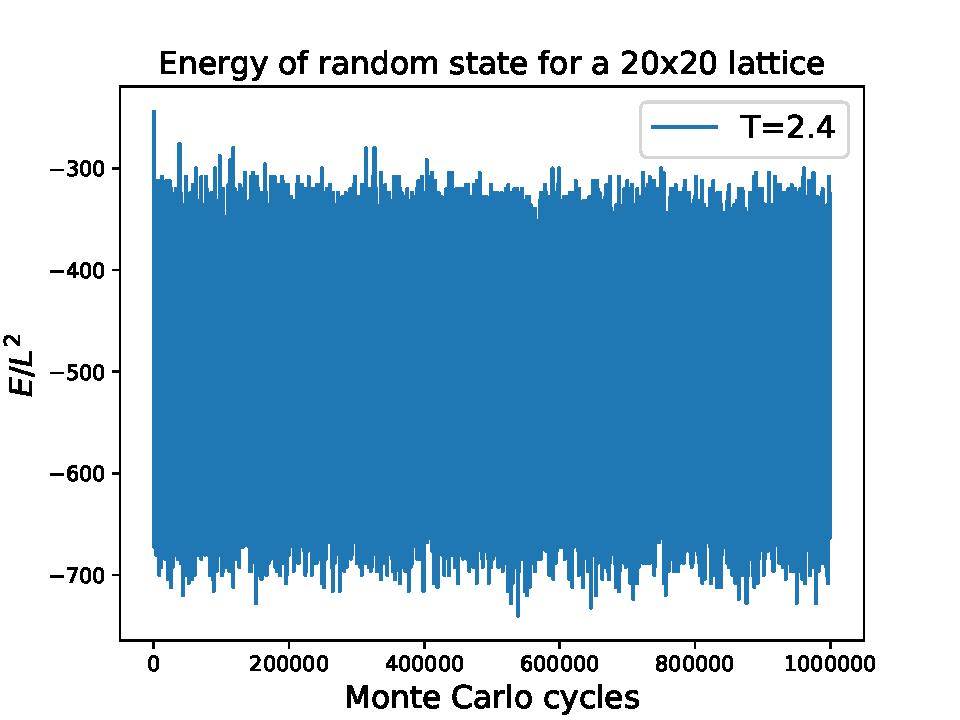
\includegraphics[width=8.65cm]{EofMCC-T2_4-L20-1e6.pdf}
  \label{fig:L20-E-T2.4}} \\
\subfloat[Absolute value of the magnetic moment pr. spin.]{ 
  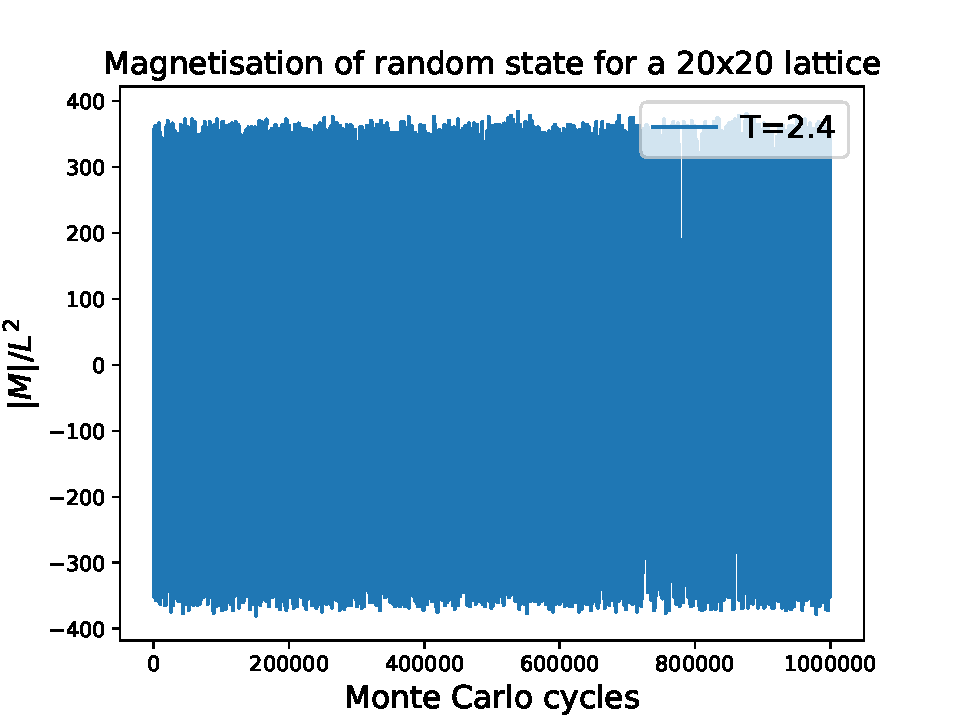
\includegraphics[width=8.65cm]{MofMCC-T2_4-L20-1e6.pdf}
  \label{fig:L20-M-T2.4}}
\caption{Time evolution (MC cycles) of energy and magnetic moment of an random initial state with temperature 2.4 kT/J. $10^6$ Monte Carlo cycles.}
\label{fig:EM-T2.4}
\end{figure}

\subsection{Accepted states in the Metropolis algorithm}
The accepted states as a function of temperature and MC cycles are found in figures \ref{fig:logAccepts(t)} and \ref{fig:logAccepts} respectively, both are logarithmic plots.
\begin{figure}
\mbox{\epsfig{figure=accepts_of_T-T1T2_4-L20.pdf,width=\linewidth,clip=}}
\caption{Logarithm of the accepted states as a function of the temperature for different number of Monte Carlo cycles. The left four dots corresponds to $T=1$ kT/J, and the right four dots corresponds to $T=2.4$ kT/J. The initial spins are randomly organized.}
\label{fig:logAccepts(t)}
\end{figure}
\begin{figure}
\mbox{\epsfig{figure=accepts-T1T2_4-L20-1e5.pdf,width=\linewidth,clip=}}
\caption{Logarithmic plot of accepted states as a function of Monte Carlo cycles. The initial spins are randomly organized.}
\label{fig:logAccepts}
\end{figure}

\subsection{Probability of energy}
In figures \ref{fig:histT1} and \ref{fig:histT2.4} we can see the probability distribution for a given energy for temperature 1 kT/J and 2.4 kT/J respectively. The variance of the energy $\sigma_E^2 = 9.398$ for temperature 1 kT/J and $\sigma_E^2 = 3264.7$ for temperature 2.4 kT/J.
%
\begin{figure}
\mbox{\epsfig{figure=PE-T1-L20-1e6.pdf,width=\linewidth,clip=}}
\caption{Histogram of the probability as a function of energy. Temperature is 1 kT/J. Initial spin states are random. 1e6 MC cycles.}
\label{fig:histT1}
\end{figure}
%
\begin{figure}
\mbox{\epsfig{figure=PE-T2_4-L20-1e6.pdf,width=\linewidth,clip=}}
\caption{Histogram of the probability as a function of energy. Temperature is 2.4 kT/J. Initial spin states are random. 1e6 MC cycles.}
\label{fig:histT2.4}
\end{figure}

\subsection{Varying temperature}
\begin{figure}
\mbox{\epsfig{figure=E-T2-23.pdf,width=\linewidth,clip=}}
\caption{Mean energy pr. spin for various lattice sizes. $10^6$ MC cycles. Initial spin state is random. Temperature varies with a step size of 0.03, making it ten steps.}
\label{fig:E-T2-23}
\end{figure}
%
\begin{figure}
\mbox{\epsfig{figure=M-T2-23.pdf,width=\linewidth,clip=}}
\caption{Mean absolute value of magnetic moment pr. spin for various amounts of MC cycles. Initial spin state is random. Temperature varies with a step size of 0.03, making it ten steps.}
\label{fig:M-T2-23}
\end{figure}
%
\begin{figure}
\mbox{\epsfig{figure=CV-T2-23.pdf,width=\linewidth,clip=}}
\caption{Heat capacity pr. spin for various lattice sizes. $10^6$ MC cycles. Initial spin state is random. Temperature varies with a step size of 0.03, making it ten steps.}
\label{fig:CV-T2-23}
\end{figure}
%
\begin{figure}
\mbox{\epsfig{figure=X-T2-23.pdf,width=\linewidth,clip=}}
\caption{Susceptibility pr. spin for various lattice sizes. $10^6$ MC cycles.. Initial spin state is random. Temperature varies with a step size of 0.03, making it ten steps.}
\label{fig:chi-T2-23}
\end{figure}
%
\begin{figure}
\mbox{\epsfig{figure=E-T22-24.pdf,width=\linewidth,clip=}}
\caption{Mean energy pr. spin for various lattice sizes. $10^6$ MC cycles. Initial spin state is random. Temperature varies with a step size of 0.01, making it twenty steps.}
\label{fig:E-T22-23}
\end{figure}
%
\begin{figure}
\mbox{\epsfig{figure=M-T22-24.pdf,width=\linewidth,clip=}}
\caption{Mean abslute value of the magnetic moment pr. spin for various lattice sizes. $10^6$ MC cycles.. Initial spin state is random. Temperature varies with a step size of 0.01, making it twenty steps.}
\label{fig:M-T22-23}
\end{figure}
%
\begin{figure}
\mbox{\epsfig{figure=CV-T22-24.pdf,width=\linewidth,clip=}}
\caption{Heat capacity pr. spin for various lattice sizes. $10^6$ MC cycles.. Initial spin state is random. Temperature varies with a step size of 0.01, making it twenty steps.}
\label{fig:CV-T22-24}
\end{figure}
%
\begin{figure}
\mbox{\epsfig{figure=X-T22-24.pdf,width=\linewidth,clip=}}
\caption{Susceptibility pr. spin for various lattice sizes. $10^6$ MC cycles. Initial spin state is random. Temperature varies with a step size of 0.01, making it twenty steps.}
\label{fig:chi-T22-23}
\end{figure}
%
In figures \ref{fig:E-T2-23}-\ref{fig:chi-T2-23} we can see plots of mean energy, mean magnetisation, heat capacity and susceptibility as a function of temperature. The temperature varies from 2-2.3 kT/J. The number of MC cycles are $10^6$, with a random initial state for the spins. In figures \ref{fig:E-T22-23}-\ref{fig:chi-T22-23} the temperature interval and temperature step are changed to $2.2-2.4$ kT/J and $0.01$ respectively, this is done to focus on the temperature where we expect to find the critical temperature. 


\subsection{Critical temperature}
\begin{figure}
\mbox{\epsfig{figure=FittedTc.pdf,width=\linewidth,clip=}}
\caption{Linear regression used on the critical temperatures at points of 1/L for $L = 40$, $60$, $80$ and $100$ gives the function $y(x) = 1.586x + 2.256$.}
\label{fig:FittedTc}
\end{figure}
%
Figure \ref{fig:FittedTc} the critical temperature as a function of 1/L is plottet. Critical temperature was extracted from the susceptibility plotted in figure \ref{fig:chi-T22-23}, that is; we have extracted the corresponding temperature of the highest value of the susceptibility. Linear regression gives the function $y(x) = 1.586x + 2.256$. When $L \rightarrow \infty$, this corresponds to $1/L \rightarrow 0$. We can see that $y(0) = 2.256$, which is the numerical value for the critical temperature when the lattice size $L \rightarrow \infty$.


\subsection{Run times}
In table \ref{tab:runtimes40} and \ref{tab:runtimes100} the runes times for a 40x40 and a 100x100 lattice, respectively. 
%
\begin{deluxetable}{cccc}
\tablewidth{0pt}
\tablecaption{\label{tab:runtimes40}}
\tablecomments{Run times for a 40x40 lattice for $10^5$ Monte Carlo cycles. Temperature set to 1 kT/J and the initial state for the spins are random. The machine that has been used for the calculations has two cores, where each core has two threads, making up a total of four threads.}
\tablecolumns{4}
\tablehead{Run & 1 thread & 4 threads & Difference}
\startdata
1 & 13.910 & 4.448 & 9.461 \\
2 & 14.348 & 4.530 & 9.817 \\
3 & 14.407 & 4.636 & 9.770 \\
Average & 14.221 & 4.538 & 9.683
\enddata
\end{deluxetable}
%
\begin{deluxetable}{cccc}
\tablewidth{0pt}
\tablecaption{\label{tab:runtimes100}}
\tablecomments{Run times for a 100x100 lattice for $10^5$ Monte Carlo cycles. Temperature set to 1 kT/J and the initial state for the spins are random.}
\tablecolumns{5}
\tablehead{Run & 1 core & 4 core & Difference}
\startdata
1 & 91.137 & 34.434 & 62.702 \\
2 & 83.662 & 30.455 & 53.207 \\
3 & 86.905 & 28.534 & 58.371 \\
Average & 87.235 & 31.141 & 58.093
\enddata
\end{deluxetable}






\section{Discussion}
\label{sec:discussion}
 When comparing the analytical and the numerical values for a 2x2 lattice we can see in Table \ref{tab:numAnal} that the numerical values for the mean energy and mean absolute value of the magnetic moment are fairly stable, and does not deviate much from the analytical values, even for few MC cycles. At MC cycles less than 10000 we see that the results fluctuate, and after they have stabilized.
 
 In the figures \ref{fig:EM-GS-T1} and \ref{fig:EM-GS-T2.4} showing the energy and magnetic moment for the ground state (i.e. ordered initial state) for temperature 1 and 2.4 kT/J respectively, shows that the system stabilizes quickly. We expect the system to stabilize quickly due to the fact that the initial state in the most likely state. For the low temperature situation there are few states where the energy of the system increases. 
 
 If we start the system in a random spin state the system takes some time to stabilize, as shown in figure \ref{fig:EM-T1_zoom}, a zoom of figure \ref{fig:EM-T1}, for the low temperature. For the increased temperature we see in figure \ref{fig:EM-T2.4} that the stable state of the system have much higher amplitudes of the energy and the magnetisation than that of the lower temperature, since there is more energy present in the system. 
 %
 From the probability distribution, Eq. \eqref{eq:P_i}, we see that 
 %
 \begin{align*}
 P_i \propto e^{-\beta E_i} = e^{-E_i/kT} \propto e^{-1/T}
 \end{align*}
 %
 for a state with energy $E_i$. So the probability of a state with the energy $E_i$ increases with the temperature. In the case of the higher temperature, the probability of reaching a state with a higher energy is increased. In figure \ref{fig:EM-T2.4} we see that there are more states with higher energies, which is a direct result from increasing the temperature, and therefore the energy of the system. Looking at the accepted states as a function of MC cycles shown in figure \ref{fig:logAccepts} and \ref{fig:logAccepts(t)} we can see that there are more accepted states for the case where the system has the highest temperature. Further we see in the histograms in figure \ref{fig:histT1} and \ref{fig:histT2.4} that the system has more states with with varying energy when the temperature is higher.
 
Studying the Ising model as the temperature of the system increases we see in figure \ref{fig:E-T2-23}-\ref{fig:chi-T2-23} that the system is stable, and there is not much happening, so the model of 40x40 lattice is sufficient. When the temperature reaches $\sim 2.20-2.23$ the temperature has reached the analytical value of the critical temperature, which suggests a phase transition. In figures \ref{fig:E-T22-23} and \ref{fig:chi-T22-23} the temperature interval is from $2.2-2.4$, and the resolution of the temperature is increased. The figures shows that there is a phase transition, which depends on the lattice size. In figure \ref{fig:chi-T22-23} we can see that the peak of the susceptibility and the heat capacity spikes as we increase the lattice size, which is expected for the Ising model. Further increasing the lattice size we would expect sharper and taller peak, and as $L\rightarrow \infty$ we expect $\chi$, $C_V \rightarrow \infty$. Extracting the values of the peak from the susceptibility we use linear regression to find the value of the critical temperature as $L\rightarrow \infty \Longleftrightarrow 1/L \rightarrow 0$, the function is shown in figure \ref{fig:FittedTc}.
When increasing the lattice size, we can see from figures \ref{fig:E-T2-23}-\ref{fig:chi-T22-23} that this corresponds to increasing the resolution of our calculation, which is what one would expect, considering that we are getting a better approximation of a real magnetic system when increasing the lattice size. 
When parallelising our software we gain a significant speed up, as shown in Table \ref{tab:runtimes40} and \ref{tab:runtimes100}. The speed up does not decrease by a factor four if running four processes, due to each run having to prepare and do a clean up for each run. 

\section{Conclusions}
\label{sec:conclusions}
The Ising model for a finite lattice proves to give a good estimate of the analytical value of the critical temperature, which is the temperature of which a magnetic system undergoes a phase transformation. Increasing the lattice size gives a better approximations and a more realistic model, increasing it further than what has been done in this study will allow for a better approximation of the critical temperature. The figures provided for the mean energy and magnetisation, the heat capacity and the susceptibility shows a consistent behavior of a phase transition for a temperature $\sim T_C$. 

\begin{thebibliography}{}
\bibitem{bib:onsager} 
Onsager, Lars,
 \textit{Crystal Statistics. I. A Two-Dimensional Model with an Order-Disorder Transition}
\url{https://link.aps.org/doi/10.1103/PhysRev.65.117}

\end{thebibliography}



\end{document}
